% answers.tex —— 2010 年·全国新课标卷·文科 · 参考答案与详细解析片段
% 由 tools/generate_projects.py 依来源总账自 2010/2010_数学真题_全国新课标文_试题.md + 2010/2010_数学真题_全国新课标文_解析正文.md + 2010/2010_数学真题_全国新课标文_答案要点.md 生成，勿手改（改源 MD 后重跑）


\begin{answer}
\gksolhead{1}{}

\textbf{题目}：

已知集合 $A=\{x\mid |x|\leq2,\ x\in\mathbb R\}$，$B=\{x\mid x\leq4,\ x\in\mathbb Z\}$，则 $A\cap B=$\mbox{（　　）}

（A）$(0,2)$\quad（B）$[0,2]$\quad（C）$\{0,2\}$\quad（D）$\{0,1,2\}$

\Needspace{4\baselineskip}
\textbf{解析}

$A\cap B=\{0,1,2\}$，选 D。

\gkanswer{答案：D}

\end{answer}
\begin{answer}
\gksolhead{2}{}

\textbf{题目}：

已知 $\boldsymbol a\text{、}\boldsymbol b$ 为平面向量，若 $\boldsymbol a=(4,3)$，$2\boldsymbol a+\boldsymbol b=(3,18)$，则 $\boldsymbol a\text{、}\boldsymbol b$ 夹角的余弦值等于\mbox{（　　）}

（A）$\dfrac8{65}$\quad（B）$-\dfrac8{65}$\quad（C）$\dfrac{16}{65}$\quad（D）$-\dfrac{16}{65}$

\Needspace{4\baselineskip}
\textbf{解析}

\Needspace{5\baselineskip}
$\boldsymbol b=(3,18)-2(4,3)=(-5,12)$，故
\nopagebreak[4]
\[
\cos\theta=\frac{4(-5)+3(12)}{5\cdot13}=\frac{16}{65}\text{，}
\]
选 C。

\gkanswer{答案：C}

\end{answer}
\begin{answer}
\gksolhead{3}{}

\textbf{题目}：

已知复数 $z=\left(\dfrac{\sqrt3+i}{1-\sqrt3i}\right)^2$，则 $|z|=$\mbox{（　　）}

（A）$\dfrac14$\quad（B）$\dfrac12$\quad（C）$1$\quad（D）$2$

\Needspace{4\baselineskip}
\textbf{解析}

括号内复数的模为 $1$，平方后仍有 $|z|=1$，选 C。

\gkanswer{答案：C}

\end{answer}
\begin{answer}
\gksolhead{4}{}

\textbf{题目}：

曲线 $y=x^3-2x+1$ 在点 $(1,0)$ 处的切线方程为\mbox{（　　）}

（A）$y=x-1$\quad（B）$y=-x+1$\quad（C）$y=2x-2$\quad（D）$y=-2x+2$

\Needspace{4\baselineskip}
\textbf{解析}

$y'=3x^2-2$，在 $x=1$ 处斜率为 $1$，过 $(1,0)$ 的切线为 $y=x-1$，选 A。

\gkanswer{答案：A}

\end{answer}
\begin{answer}
\gksolhead{5}{}

\textbf{题目}：

中心在原点、焦点在 $x$ 轴上的双曲线的一条渐近线经过点 $(4,2)$，则它的离心率为\mbox{（　　）}

（A）$\sqrt6$\quad（B）$\sqrt5$\quad（C）$\dfrac{\sqrt6}{2}$\quad（D）$\dfrac{\sqrt5}{2}$

\Needspace{4\baselineskip}
\textbf{解析}

\Needspace{5\baselineskip}
渐近线斜率为 $2/4=1/2$，故双曲线离心率
\nopagebreak[4]
\[
e=\sqrt{1+\left(\frac12\right)^2}=\frac{\sqrt5}{2}\text{，}
\]
选 D。

\gkanswer{答案：D}

\end{answer}
\begin{answer}
\gksolhead{6}{}

\textbf{题目}：

如图，质点 $P$ 在半径为 $2$ 的圆周上逆时针运动，其初始位置为 $P_0(\sqrt2,-\sqrt2)$，角速度为 $1$，那么点 $P$ 到 $x$ 轴的距离 $d$ 关于时间 $t$ 的函数图象大致为\mbox{（　　）}
\nopagebreak[4]
\begin{center}% 2010 全国卷文科第 6 题：质点圆周运动的四个函数图象选项。
\begin{tikzpicture}[font=\scriptsize, line width=0.35pt]
  \begin{scope}[shift={(0,0)}]
    \draw[->] (0,0) -- (3.8,0) node[right] {$t$};
    \draw[->] (0,0) -- (0,2.35) node[above] {$d$};
    \draw[domain=0:3.35, samples=100, smooth, variable=\tau]
      plot (\tau,{2*abs(sin(deg(\tau)))});
    \node[below left] at (0,0) {O}; \node at (0.2,2.55) {A};
  \end{scope}
  \begin{scope}[shift={(4.9,0)}]
    \draw[->] (0,0) -- (3.8,0) node[right] {$t$};
    \draw[->] (0,0) -- (0,2.35) node[above] {$d$};
    \draw[domain=0:3.35, samples=100, smooth, variable=\tau]
      plot (\tau,{2*abs(sin(deg(\tau+45)))});
    \node[below left] at (0,0) {O}; \node at (0.2,2.55) {B};
  \end{scope}
  \begin{scope}[shift={(0,-3.0)}]
    \draw[->] (0,0) -- (3.8,0) node[right] {$t$};
    \draw[->] (0,0) -- (0,2.35) node[above] {$d$};
    \draw[domain=0:3.35, samples=100, smooth, variable=\tau]
      plot (\tau,{2*abs(sin(deg(\tau-45)))});
    \node[below left] at (0,0) {O}; \node at (0.2,2.55) {C};
  \end{scope}
  \begin{scope}[shift={(4.9,-3.0)}]
    \draw[->] (0,0) -- (3.8,0) node[right] {$t$};
    \draw[->] (0,0) -- (0,2.35) node[above] {$d$};
    \draw[domain=0:3.35, samples=100, smooth, variable=\tau]
      plot (\tau,{2*abs(cos(deg(\tau)))});
    \node[below left] at (0,0) {O}; \node at (0.2,2.55) {D};
  \end{scope}
\end{tikzpicture}
\end{center}
\nopagebreak[4]
（A）图 A\quad（B）图 B\quad（C）图 C\quad（D）图 D

\Needspace{4\baselineskip}
\textbf{解析}

初始角为 $-\pi/4$，点到 $x$ 轴的距离为
$d(t)=2|\sin(t-\pi/4)|$，从 $\sqrt2$ 开始下降并在 $t=\pi/4$ 首次为零，选 C。

\gkanswer{答案：C}

\end{answer}
\begin{answer}
\gksolhead{7}{}

\textbf{题目}：

设长方体的长、宽、高分别为 $2a\text{、}a\text{、}a$，其顶点都在一个球面上，则该球的表面积为\mbox{（　　）}

（A）$3\pi a^2$\quad（B）$6\pi a^2$\quad（C）$12\pi a^2$\quad（D）$24\pi a^2$

\Needspace{4\baselineskip}
\textbf{解析}

\Needspace{5\baselineskip}
长方体外接球半径满足
\nopagebreak[4]
\[
R^2=\frac{(2a)^2+a^2+a^2}{4}=\frac{3a^2}{2}\text{，}
\]
故球表面积为 $4\pi R^2=6\pi a^2$，选 B。

\gkanswer{答案：B}

\end{answer}
\begin{answer}
\gksolhead{8}{}

\textbf{题目}：

如果执行如图所示的框图，输入 $N=5$，则输出的数等于\mbox{（　　）}
\nopagebreak[4]
\begin{center}% 2010 全国卷文科第 8 题：程序框图。
\begin{tikzpicture}[font=\footnotesize, >=Stealth, node distance=2.2mm, line width=0.4pt,
  box/.style={draw, minimum height=1.5em, minimum width=5.8em, inner xsep=6pt},
  term/.style={draw, rounded corners=6pt, minimum height=1.5em, inner xsep=8pt},
  io/.style={draw, trapezium, trapezium left angle=70, trapezium right angle=110,
             minimum height=1.5em, inner xsep=3pt},
  dec/.style={draw, diamond, aspect=2.6, inner sep=1.5pt}]
  \node[term] (start) {开始};
  \node[io, below=of start] (input) {输入 $N$};
  \node[box, below=of input] (init) {$k=1,\ S=0$};
  \node[box, below=of init] (step) {$S=S+\dfrac{1}{k(k+1)}$};
  \node[dec, below=of step] (cond) {$k<N$};
  \node[box, right=16mm of cond] (inc) {$k=k+1$};
  \node[io, below=9mm of cond] (output) {输出 $S$};
  \node[term, below=of output] (end) {结束};
  \draw[->] (start) -- (input);
  \draw[->] (input) -- (init);
  \draw[->] (init) -- (step);
  \draw[->] (step) -- (cond);
  \draw[->] (cond.east) -- node[above] {是} (inc.west);
  \draw[->] (inc.north) |- (step.east);
  \draw[->] (cond.south) -- node[right] {否} (output.north);
  \draw[->] (output) -- (end);
\end{tikzpicture}
\end{center}
\nopagebreak[4]
（A）$\dfrac54$\quad（B）$\dfrac45$\quad（C）$\dfrac65$\quad（D）$\dfrac56$

\Needspace{4\baselineskip}
\textbf{解析}

流程图在每次累加后判断 $k<N$，若为真才令 $k=k+1$ 并继续循环。输入
\Needspace{5\baselineskip}
$N=5$ 时累加 $k=1,2,3,4,5$，故
\nopagebreak[4]
\[
S=\sum_{k=1}^5\frac1{k(k+1)}=1-\frac16=\frac56\text{，}
\]
选 D。

\gkanswer{答案：D}

\end{answer}
\begin{answer}
\gksolhead{9}{}

\textbf{题目}：

设偶函数 $f(x)$ 满足 $f(x)=2^x-4$（$x\geq0$），则 $\{x\mid f(x-2)>0\}=$\mbox{（　　）}

（A）$\{x\mid x<-2\text{ \text{或} }x>4\}$\quad（B）$\{x\mid x<0\text{ \text{或} }x>4\}$

（C）$\{x\mid x<0\text{ \text{或} }x>6\}$\quad（D）$\{x\mid x<-2\text{ \text{或} }x>2\}$

\Needspace{4\baselineskip}
\textbf{解析}

因 $f$ 为偶函数，$f(x-2)=2^{|x-2|}-4$。不等式等价于
$|x-2|>2$，解集为 $x<0$ 或 $x>4$，选 B。

\gkanswer{答案：B}

\end{answer}
\begin{answer}
\gksolhead{10}{}

\textbf{题目}：

若 $\cos\alpha=-\dfrac45$，$\alpha$ 是第三象限的角，则 $\sin\left(\alpha+\dfrac\pi4\right)=$\mbox{（　　）}

（A）$-\dfrac{7\sqrt2}{10}$\quad（B）$\dfrac{7\sqrt2}{10}$\quad（C）$-\dfrac{\sqrt2}{10}$\quad（D）$\dfrac{\sqrt2}{10}$

\Needspace{4\baselineskip}
\textbf{解析}

\Needspace{5\baselineskip}
第三象限中 $\sin\alpha=-3/5$，所以
\nopagebreak[4]
\[
\sin\left(\alpha+\frac\pi4\right)
=\frac{-3-4}{5\sqrt2}=-\frac{7\sqrt2}{10}\text{，}
\]
选 A。

\gkanswer{答案：A}

\end{answer}
\begin{answer}
\gksolhead{11}{}

\textbf{题目}：

已知平行四边形 $ABCD$ 的三个顶点为 $A(-1,2)\text{、}B(3,4)\text{、}C(4,-2)$，点 $(x,y)$ 在平行四边形 $ABCD$ 的内部，则 $z=2x-5y$ 的取值范围是\mbox{（　　）}

（A）$(-14,16)$\quad（B）$(-14,20)$\quad（C）$(-12,18)$\quad（D）$(-12,20)$

\Needspace{4\baselineskip}
\textbf{解析}

平行四边形第四个顶点为 $D=A+C-B=(0,-4)$。在四个顶点处
$2x-5y$ 的值分别为 $-12,-14,18,20$，内部取值范围为 $(-14,20)$，选 B。

\gkanswer{答案：B}

\end{answer}
\begin{answer}
\gksolhead{12}{}

\textbf{题目}：

\Needspace{5\baselineskip}
已知函数

\nopagebreak[4]
\[
f(x)=\begin{cases}|\lg x|,&0<x\leq10,\\-\dfrac12x+6,&x>10,\end{cases}
\]

若 $a\text{、}b\text{、}c$ 互不相等，且 $f(a)=f(b)=f(c)$，则 $abc$ 的取值范围是\mbox{（　　）}

（A）$(1,10)$\quad（B）$(5,6)$\quad（C）$(10,12)$\quad（D）$(20,24)$

\Needspace{4\baselineskip}
\textbf{解析}

令公共函数值为 $t\in(0,1)$。三个原像为 $10^{-t}$、$10^t$ 和
\Needspace{5\baselineskip}
$12-2t$，故
\nopagebreak[4]
\[
abc=12-2t\in(10,12)\text{，}
\]
选 C。

\gkanswer{答案：C}

\end{answer}
\begin{answer}
\gksolhead{13}{}

\textbf{题目}：

圆心位于原点且与直线 $x+y-2=0$ 相切的圆的方程为\gkblank{}。

\Needspace{4\baselineskip}
\textbf{解析}

\Needspace{5\baselineskip}
圆心为原点，且到直线 $x+y-2=0$ 的距离为 $\sqrt2$，故方程为
\nopagebreak[4]
\[x^2+y^2=2.\]

\gkanswer{答案：$x^2+y^2=2$}

\end{answer}
\begin{answer}
\gksolhead{14}{}

\textbf{题目}：

设函数 $y=f(x)$ 在区间 $[0,1]$ 上的图象是连续不断的一条曲线，且恒有 $0\leq f(x)\leq1$。用随机模拟方法近似计算由曲线、$x=0$、$x=1$、$y=0$ 所围成部分的面积 $S$，先产生两组（每组 $N$ 个）区间 $[0,1]$ 上的均匀随机数 $x_i\text{、}y_i$，数出满足 $y_i\leq f(x_i)$ 的点数 $N_1$，则 $S$ 的近似值为\gkblank{}。

\Needspace{4\baselineskip}
\textbf{解析}

\Needspace{5\baselineskip}
单位正方形中满足 $y_i\leq f(x_i)$ 的点占比近似所围面积，因此
\nopagebreak[4]
\[S\approx\frac{N_1}{N}.
\]

\gkanswer{答案：$\dfrac{N_1}{N}$}

\end{answer}
\begin{answer}
\gksolhead{15}{}

\textbf{题目}：

一个几何体的正视图为一个三角形，则这个几何体可能是下列几何体中的（填入所有可能的几何体前的编号）：①三棱锥　②四棱锥　③三棱柱　④四棱柱　⑤圆锥　⑥圆柱。答案为\gkblank{}。

\Needspace{4\baselineskip}
\textbf{解析}

三棱锥、四棱锥和圆锥均可选择合适的放置方向，使正视图为三角形，故填
①②⑤。

\gkanswer{答案：①②⑤}

\end{answer}
\begin{answer}
\gksolhead{16}{}

\textbf{题目}：

在 $\triangle ABC$ 中，$D$ 为 $BC$ 边上一点，$BC=3BD$，$AD=\sqrt2$，$\angle ADB=135^\circ$。若 $AC=\sqrt2 AB$，则 $BD=$\gkblank{}。

\Needspace{4\baselineskip}
\textbf{解析}

令 $BD=x$，则 $DC=2x$。由 $AD=\sqrt2$、$\angle ADB=135^\circ$、
\Needspace{5\baselineskip}
$\angle ADC=45^\circ$，余弦定理给出
\nopagebreak[4]
\[
AB^2=x^2+2+2x\text{，}\qquad AC^2=4x^2-4x+2.
\]
\Needspace{5\baselineskip}
又 $AC=\sqrt2 AB$，所以
\nopagebreak[4]
\[
4x^2-4x+2=2(x^2+2+2x)\text{，}
\]
\Needspace{5\baselineskip}
即 $x^2-4x-1=0$。因 $x>0$，取正根得
\nopagebreak[4]
\[
BD=x=2+\sqrt5.
\]

\gkanswer{答案：$2+\sqrt5$}

\end{answer}
\begin{answer}
\gksolhead{17}{}

\textbf{题目}：

设等差数列 $\{a_n\}$ 满足 $a_3=5$，$a_{10}=-9$。

（1） 求 $\{a_n\}$ 的通项公式；

（2） 求 $\{a_n\}$ 的前 $n$ 项和 $S_n$ 及使得 $S_n$ 最大的序号 $n$ 的值。

\Needspace{4\baselineskip}
\textbf{解析}

\gksubpart{(1)}

\Needspace{5\baselineskip}
由 $a_3=5$、$a_{10}=-9$ 得公差 $d=-2$、$a_1=9$，所以
\nopagebreak[4]
\[a_n=11-2n.
\]

\gksubpart{(2)}

\nopagebreak[4]
\[
S_n=\frac n2(9+11-2n)=n(10-n)=25-(n-5)^2\text{，}
\]
故最大时 $n=5$。

\gkanswer{答案（1）：$a_n=11-2n$。}

\gkanswer{答案（2）：$S_n=n(10-n)$，$S_n$ 最大时 $n=5$。}

\end{answer}
\begin{answer}
\gksolhead{18}{}

\textbf{题目}：

如图，已知四棱锥 $P-ABCD$ 的底面为等腰梯形，$AB\parallel CD$，$AC\perp BD$，垂足为 $H$，$PH$ 是四棱锥的高。
\nopagebreak[4]
\begin{center}% 2010 全国卷文科第 18 题：等腰梯形底面的四棱锥示意图。
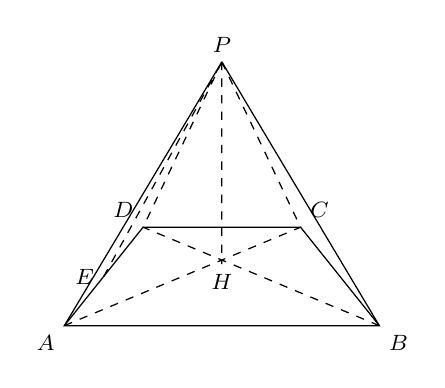
\begin{tikzpicture}[font=\footnotesize, line width=0.45pt]
  \coordinate (A) at (0,0);
  \coordinate (B) at (4.0,0);
  \coordinate (D) at (1.0,1.25);
  \coordinate (C) at (3.0,1.25);
  \coordinate (H) at (2.0,0.78);
  \coordinate (P) at (2.0,3.35);
  \coordinate (E) at (0.5,0.625);
  \draw (A)--(B)--(C)--(D)--cycle;
  \draw[dashed] (A)--(C) (B)--(D) (P)--(H) (P)--(D) (P)--(C) (E)--(P);
  \draw (P)--(A) (P)--(B);
  \node[below left] at (A) {$A$};
  \node[below right] at (B) {$B$};
  \node[above left] at (D) {$D$};
  \node[above right] at (C) {$C$};
  \node[above] at (P) {$P$};
  \node[below] at (H) {$H$};
  \node[left] at (E) {$E$};
\end{tikzpicture}
\end{center}
\nopagebreak[4]
（1） 证明：平面 $PAC\perp$ 平面 $PBD$；

（2） 若 $AB=\sqrt6$，$\angle APB=\angle ADB=60^\circ$，求四棱锥 $P-ABCD$ 的体积。

\Needspace{4\baselineskip}
\textbf{解析}

\gksubpart{(1)}

由 $AC\perp BD$ 且 $PH\perp$ 底面，得 $AC\perp PH$；又 $AC\perp BD$，
\Needspace{5\baselineskip}
故 $AC\perp$ 平面 $PBD$，从而
\nopagebreak[4]
\[\text{\text{平面} }PAC\perp\text{\text{平面} }PBD.
\]

\gksubpart{(2)}

设 $AB=L=\sqrt6$、$CD=l$、梯形高为 $h$，令 $u=(L-l)/2$。对称放置底面后，
由 $AC\perp BD$ 得 $h=(L+l)/2$；由 $\angle ADB=60^\circ$ 得
\Needspace{5\baselineskip}
$u/h=2-\sqrt3$。于是
\nopagebreak[4]
\[
CD=\sqrt2,\qquad h=\frac{\sqrt6+\sqrt2}{2},
\]
底面积为 $2+\sqrt3$。

\Needspace{5\baselineskip}
由 $\angle APB=60^\circ$ 和对称性得 $PH=\sqrt3$，故体积为
\nopagebreak[4]
\[
V=\frac13(2+\sqrt3)\sqrt3=1+\frac{2\sqrt3}{3}.
\]

\gkanswer{答案（1）：平面 $PAC\perp$ 平面 $PBD$。}

\gkanswer{答案（2）：$V=1+\dfrac{2\sqrt3}{3}$。}

\end{answer}
\begin{answer}
\gksolhead{19}{}

\textbf{题目}：

为调查某地区老人是否需要志愿者提供帮助，用简单随机抽样方法从该地区调查了 $500$ 位老年人，结果如下：

\begin{center}
\begin{tabular}{lrr}
\toprule
性别 & 男 & 女 \\
\midrule
需要 & 40 & 30 \\
不需要 & 160 & 270 \\
\bottomrule
\end{tabular}
\end{center}

（1） 估计该地区老年人中，需要志愿者提供帮助的老年人的比例；

（2） 能否有 $99\%$ 的把握认为该地区老年人是否需要志愿者提供帮助与性别有关？

（3） 根据（2）的结论，能否提供更好的调查方法来估计该地区老年人需要志愿者帮助的比例？说明理由。

\Needspace{4\baselineskip}
\textbf{解析}

\gksubpart{(1)}

\Needspace{5\baselineskip}
需要帮助的样本数为 $40+30=70$，比例估计为
\nopagebreak[4]
\[\hat p=\frac{70}{500}=0.14.
\]

\gksubpart{(2)}

\Needspace{5\baselineskip}
按源面列联表计算
\nopagebreak[4]
\[
K^2=\frac{500(40\cdot270-30\cdot160)^2}
{70\cdot430\cdot200\cdot300}\approx9.967>6.635\text{，}
\]
故有 $99\%$ 把握认为二者有关。

\gksubpart{(3)}

可按性别分层随机抽样，按总体男女比例分配样本并加权估计，提升样本代表性。

\gkanswer{答案（1）：$0.14$。}

\gkanswer{答案（2）：有 $99\%$ 的把握认为是否需要帮助与性别有关。}

\gkanswer{答案（3）：按性别分层随机抽样，再按总体比例加权估计。}

\end{answer}
\begin{answer}
\gksolhead{20}{}

\textbf{题目}：

设 $F_1\text{、}F_2$ 分别是椭圆 $E:\ x^2+\dfrac{y^2}{b^2}=1$（$0<b<1$）的左、右焦点，过 $F_1$ 的直线 $l$ 与 $E$ 相交于 $A\text{、}B$ 两点，且 $|AF_2|\text{、}|AB|\text{、}|BF_2|$ 成等差数列。

（1） 求 $|AB|$；

（2） 若直线 $l$ 的斜率为 $1$，求 $b$ 的值。

\Needspace{4\baselineskip}
\textbf{解析}

\gksubpart{(1)}

\Needspace{5\baselineskip}
椭圆长轴长为 $2$。由焦点定义及等差条件，
\nopagebreak[4]
\[
|AF_2|+|BF_2|=2|AB|,
\qquad |AF_2|+|BF_2|=4-|AB|\text{，}
\]
所以 $|AB|=4/3$。

\gksubpart{(2)}

\Needspace{5\baselineskip}
过 $F_1$ 且斜率为 $1$ 的弦与椭圆联立，弦长为
\nopagebreak[4]
\[
|AB|=\frac{4b^2}{1+b^2}.
\]
代入 $|AB|=4/3$ 得 $b^2=1/2$，故 $b=\sqrt2/2$。

\gkanswer{答案（1）：$|AB|=\dfrac43$。}

\gkanswer{答案（2）：$b=\dfrac{\sqrt2}{2}$。}

\end{answer}
\begin{answer}
\gksolhead{21}{}

\textbf{题目}：

设函数 $f(x)=x(e^x-1)-ax^2$。

（1） 若 $a=\dfrac12$，求 $f(x)$ 的单调区间；

（2） 若当 $x\geq0$ 时，$f(x)\geq0$，求 $a$ 的取值范围。

\Needspace{4\baselineskip}
\textbf{解析}

\gksubpart{(1)}

\Needspace{5\baselineskip}
当 $a=1/2$ 时
\nopagebreak[4]
\[
f'(x)=(x+1)(e^x-1)\text{，}
\]
故增区间为 $(-\infty,-1)\cup(0,+\infty)$，减区间为 $(-1,0)$。

\gksubpart{(2)}

\Needspace{5\baselineskip}
对 $x>0$，$f(x)\geq0$ 等价于
\nopagebreak[4]
\[
a\leq\frac{e^x-1}{x}.
\]
右端在 $x>0$ 上的下确界为 $1$，故 $a\leq1$。

\gkanswer{答案（1）：增区间为 $(-\infty,-1)\cup(0,+\infty)$，减区间为 $(-1,0)$。}

\gkanswer{答案（2）：$a\leq1$。}

\end{answer}
\begin{answer}
\gksolhead{22}{}

\textbf{题目}：

如图，已知圆上的弧 $\widehat{AC}=\widehat{BD}$，过 $C$ 点的圆的切线与 $BA$ 的延长线交于 $E$ 点，证明：
\nopagebreak[4]
\begin{center}% 2010 全国卷文科第 22 题：圆、切线与 BA 的延长线示意图。
\begin{tikzpicture}[font=\footnotesize, line width=0.45pt]
  \coordinate (O) at (2.25,1.85);
  \def\r{1.65}
  \coordinate (A) at (0.95,0.83);
  \coordinate (B) at (0.62,2.75);
  \coordinate (C) at (3.35,3.05);
  \coordinate (D) at (3.78,1.02);
  \coordinate (E) at (5.05,0.45);
  \draw (O) circle (\r);
  \draw (A)--(B)--(C)--(D)--cycle;
  \draw (B)--(A)--(E);
  \draw (C)--(E);
  \draw[dashed] (O)--(C);
  \node[below left] at (A) {$A$};
  \node[left] at (B) {$B$};
  \node[above right] at (C) {$C$};
  \node[below right] at (D) {$D$};
  \node[right] at (E) {$E$};
  \node[below] at (O) {$O$};
  \draw ($(C)!0.12!(E)$) -- ++(-0.17,-0.29);
\end{tikzpicture}
\end{center}
\nopagebreak[4]
（1） $\angle ACE=\angle BCD$；

（2） $BC^2=BE\cdot CD$。

\Needspace{4\baselineskip}
\textbf{解析}

\gksubpart{(1)}

\Needspace{5\baselineskip}
由切线弦定理及 $\widehat{AC}=\widehat{BD}$，得
\nopagebreak[4]
\[\angle ACE=\angle ABC=\angle BCD.
\]

\gksubpart{(2)}

\Needspace{5\baselineskip}
由共线关系和切线弦定理，$\triangle BCE\sim\triangle CDB$，故
\nopagebreak[4]
\[\frac{BE}{BC}=\frac{BC}{CD}\text{，}
\]
即 $BC^2=BE\cdot CD$。

\gkanswer{答案（1）：见解析版}

\gkanswer{答案（2）：见解析版}

\end{answer}
\begin{answer}
\gksolhead{23}{}

\textbf{题目}：

\Needspace{5\baselineskip}
已知直线 $C_1$：

\nopagebreak[4]
\[
x=1+t\cos\alpha,\qquad y=t\sin\alpha\quad(t\text{ \text{为参数}}),
\]

\Needspace{5\baselineskip}
圆 $C_2$：

\nopagebreak[4]
\[
x=\cos\theta,\qquad y=\sin\theta\quad(\theta\text{ \text{为参数}}).
\]

（1） 当 $\alpha=\dfrac\pi3$ 时，求 $C_1$ 与 $C_2$ 的交点坐标；

（2） 过坐标原点 $O$ 作 $C_1$ 的垂线，垂足为 $A$，$P$ 为 $OA$ 的中点，当 $\alpha$ 变化时，求点 $P$ 轨迹的参数方程，并指出它是什么曲线。

\Needspace{4\baselineskip}
\textbf{解析}

\gksubpart{(1)}

\Needspace{5\baselineskip}
当 $\alpha=\pi/3$ 时，代入单位圆得 $t(t+1)=0$，交点为
\nopagebreak[4]
\[
(1,0),\qquad\left(\frac12,-\frac{\sqrt3}{2}\right).
\]

\gksubpart{(2)}

\Needspace{5\baselineskip}
直线方向向量为 $(\cos\alpha,\sin\alpha)$。垂足为
\nopagebreak[4]
\[
A=(\sin^2\alpha,-\sin\alpha\cos\alpha)\text{，}
\]
\Needspace{5\baselineskip}
所以 $P$ 的参数方程为
\nopagebreak[4]
\[
x=\frac12\sin^2\alpha,\qquad y=-\frac12\sin\alpha\cos\alpha\text{，}
\]
\Needspace{5\baselineskip}
消参得
\nopagebreak[4]
\[
\left(x-\frac14\right)^2+y^2=\frac1{16}.
\]

\gkanswer{答案（1）：$(1,0)$、$\left(\dfrac12,-\dfrac{\sqrt3}{2}\right)$。}

\gkanswer{答案（2）：$x=\dfrac12\sin^2\alpha$，$y=-\dfrac12\sin\alpha\cos\alpha$；轨迹为 $\left(x-\dfrac14\right)^2+y^2=\dfrac1{16}$。}

\end{answer}
\begin{answer}
\gksolhead{24}{}

\textbf{题目}：

设函数 $f(x)=|2x-4|+1$。

（1） 画出函数 $y=f(x)$ 的图象；

（2） 若不等式 $f(x)\leq ax$ 的解集非空，求 $a$ 的取值范围。
\nopagebreak[4]
\begin{center}% 2010 全国卷文科第 24 题：y=|2x-4|+1。
\begin{tikzpicture}[font=\footnotesize, line width=0.45pt]
  \draw[->] (-0.5,0) -- (4.6,0) node[right] {$x$};
  \draw[->] (0,0) -- (0,5.4) node[above] {$y$};
  \draw[thick] (0,5) -- (2,1) -- (4.2,5.4);
  \fill (2,1) circle (1.2pt);
  \node[below] at (2,0) {$2$};
  \node[left] at (0,1) {$1$};
  \node[below left] at (0,0) {$O$};
\end{tikzpicture}
\end{center}
\nopagebreak[4]
\Needspace{4\baselineskip}
\textbf{解析}

\gksubpart{(1)}

\nopagebreak[4]
\[
f(x)=\begin{cases}5-2x,&x<2,\\2x-3,&x\geq2,\end{cases}
\]
图象为顶点 $(2,1)$ 的 V 字形折线。

\gksubpart{(2)}

对 $x<0$，$f(x)/x=5/x-2$ 的值域为 $(-\infty,-2)$；对 $x>0$，
\Needspace{5\baselineskip}
$f(x)/x$ 的最小值为 $1/2$。故存在解当且仅当
\nopagebreak[4]
\[a\in(-\infty,-2)\cup[1/2,+\infty).\]

\gkanswer{答案（1）：见解析版}

\gkanswer{答案（2）：$a\in(-\infty,-2)\cup\left[\dfrac12,+\infty\right)$。}

\end{answer}